\chapter{Σχεδίαση και Ανάλυση}

\section{Απαιτήσεις Συστήματος}




\subsection{Λειτουργικές απαιτήσεις}

Μια σειρά από λειτουργίες κρίθηκαν απαραίτητες και υλοποιηθήκαν στην παρούσα εφαρμογή. Έτσι:

\begin{itemize}
    \item Η εφαρμογή διαχείρισης του δικτύου θα πρέπει να  παρέχει στον χρήστη ένα γραφικό περιβάλλον που θα του επιτρέπει να αλληλεπιδρά εύκολα και αποδοτικά με το σύστημα. 
    \item Ο χρήστης θα πρέπει να έχει την δυνατότητα να παρακολουθεί την κατάσταση μιας συγκεκριμένης διεπαφής δικτύου, βλέποντας αν λειτουργεί σωστά ή αν υπάρχουν προβλήματα. 
    \item Επιπλέον, θα πρέπει να έχει τη δυνατότητα να βλέπει αναλυτικά στατιστικά στοιχεία για μια συγκεκριμένη δικτυακή συσκευή, όπως η χρήση δεδομένων, η ταχύτητα σύνδεσης ή τυχόν σφάλματα, αλλά και για συγκεκριμένες διεπαφές του δικτύου, ώστε να κατανοεί τη λειτουργία τους σε βάθος
    \item Η εφαρμογή θα επιτρέπει επίσης τη δημιουργία αντιγράφου ασφαλείας (\en{backup}) της τρέχουσας ρύθμισης του δικτύου, για να μπορεί ο χρήστης να επαναφέρει τη ρύθμιση αν χρειαστεί
    \item Τέλος, θα δίνεται η δυνατότητα αλλαγής της διεύθυνσης \en{IP} μιας επιλεγμένης δικτυακής εφαρμογής, εξασφαλίζοντας μεγαλύτερη ευελιξία στη διαχείριση του δικτύου. 
\end{itemize}

Όλες αυτές οι λειτουργίες έχουν σχεδιαστεί για να διευκολύνουν τη διαχείριση και την παρακολούθηση του δικτύου, ακόμα και από χρήστες χωρίς εξειδικευμένες γνώσεις.


\section{Αρχιτεκτονική της εφαρμογής}

Στην αρχή, οι εφαρμογές ιστού δεν ήταν τίποτα περισσότερο από ένα σύνολο αρχείων \en{HTML, CSS} και
\en{javascript} που ήταν συνδεδεμένα μεταξύ τους. Ένας καλός προγραμματιστής ήταν σε θέση να φτιάξει σπουδαίες εφαρμογές ιστού αν αυτός/αυτή
είχε αρκετές δεξιότητες/γνώσεις.

Στην εποχή μας, εμφανίστηκαν τα \en{frameworks} και λαμβάνοντας υπόψη ότι ουσιαστικά δεν βελτιώνουν αυτό που τελικά βλέπει ο χρήστης και τις
αλληλεπιδράσεις του με το \en{frontend}, τότε
θα μπορούσε κανείς να αναρωτηθεί γιατί χρησιμοποιούνται ευρέως στις μέρες μας.
Παρόμοιες δουλειές με την παρούσα εργασία υπάρχουν και σε άλλες διπλωματικές εργασίες καθώς και σε μη διπλωματικές εργασίες. Μηχανικοί από όλο τον κόσμο
ασχολούνται με την αυτοματοποίηση συστημάτων και τη δημιουργία κώδικα που να αυτοματοποιεί συσκευές/συστήματα. 

Με βάση άλλες τέτοιες προσπάθειες που έχουν γίνει στο παρελθόν εμείς συλλέξαμε την εως τώρα βιβλιογραφία
και προσπαθήσαμε να φτιάξουμε μία τέτοια εφαρμογή η οποία όμως να βασίζεται στα τωρινά δεδομένα και να 
ενσωματσώσουμε τις τελευταίες τεχνολογίες αιχμής όπως την \en{Cloud Native} αρχιτεκτονική. Στη συνέχεια γίνεται προσπάθεια να δωθεί εκτενής
ανάλυση στο πως λειτουργεί η εφαρμογή καθώς και στην αλληλλεπίδρασή της με τα συνεργαζόμενα συστήματα. 
 
\subsection{Μοντέλο \en{MVC} (\en{Model-View-Controller})}

Το μοτίβο \en{MVC}[15] (\en{Model-View-Controller} σχήμα 5.1) είναι ένα αρχιτεκτονικό πρότυπο ανάπτυξης λογισμικού που έχει ως στόχο τον διαχωρισμό της παρουσίασης των δεδομένων από τη λογική που διέπει τη διαχείριση των αλληλεπιδράσεων του χρήστη. Συγκεκριμένα, το \en{"Model"} αναλαμβάνει τη διαχείριση των δεδομένων και της επιχειρησιακής λογικής, το "\en{View}" είναι υπεύθυνο για την παρουσίαση των δεδομένων στον χρήστη, ενώ το "\en{Controller}" χειρίζεται την αλληλεπίδραση του χρήστη και τη ροή των δεδομένων μεταξύ του \en{Model} και του \en{View}.
Χάρη στη δομή του, το \en{MVC} προσφέρει μεγαλύτερη ευελιξία, επεκτασιμότητα και καλύτερη οργάνωση του κώδικα, καθιστώντας το ιδανικό για σύνθετες εφαρμογές. Γι’ αυτόν τον λόγο, όλα τα κορυφαία \en{frameworks} για την ανάπτυξη εφαρμογών \en{web}, όπως το \en{Django}, είναι βασισμένα σε αυτό το μοτίβο.


\begin{figure}[h]
	\centering
	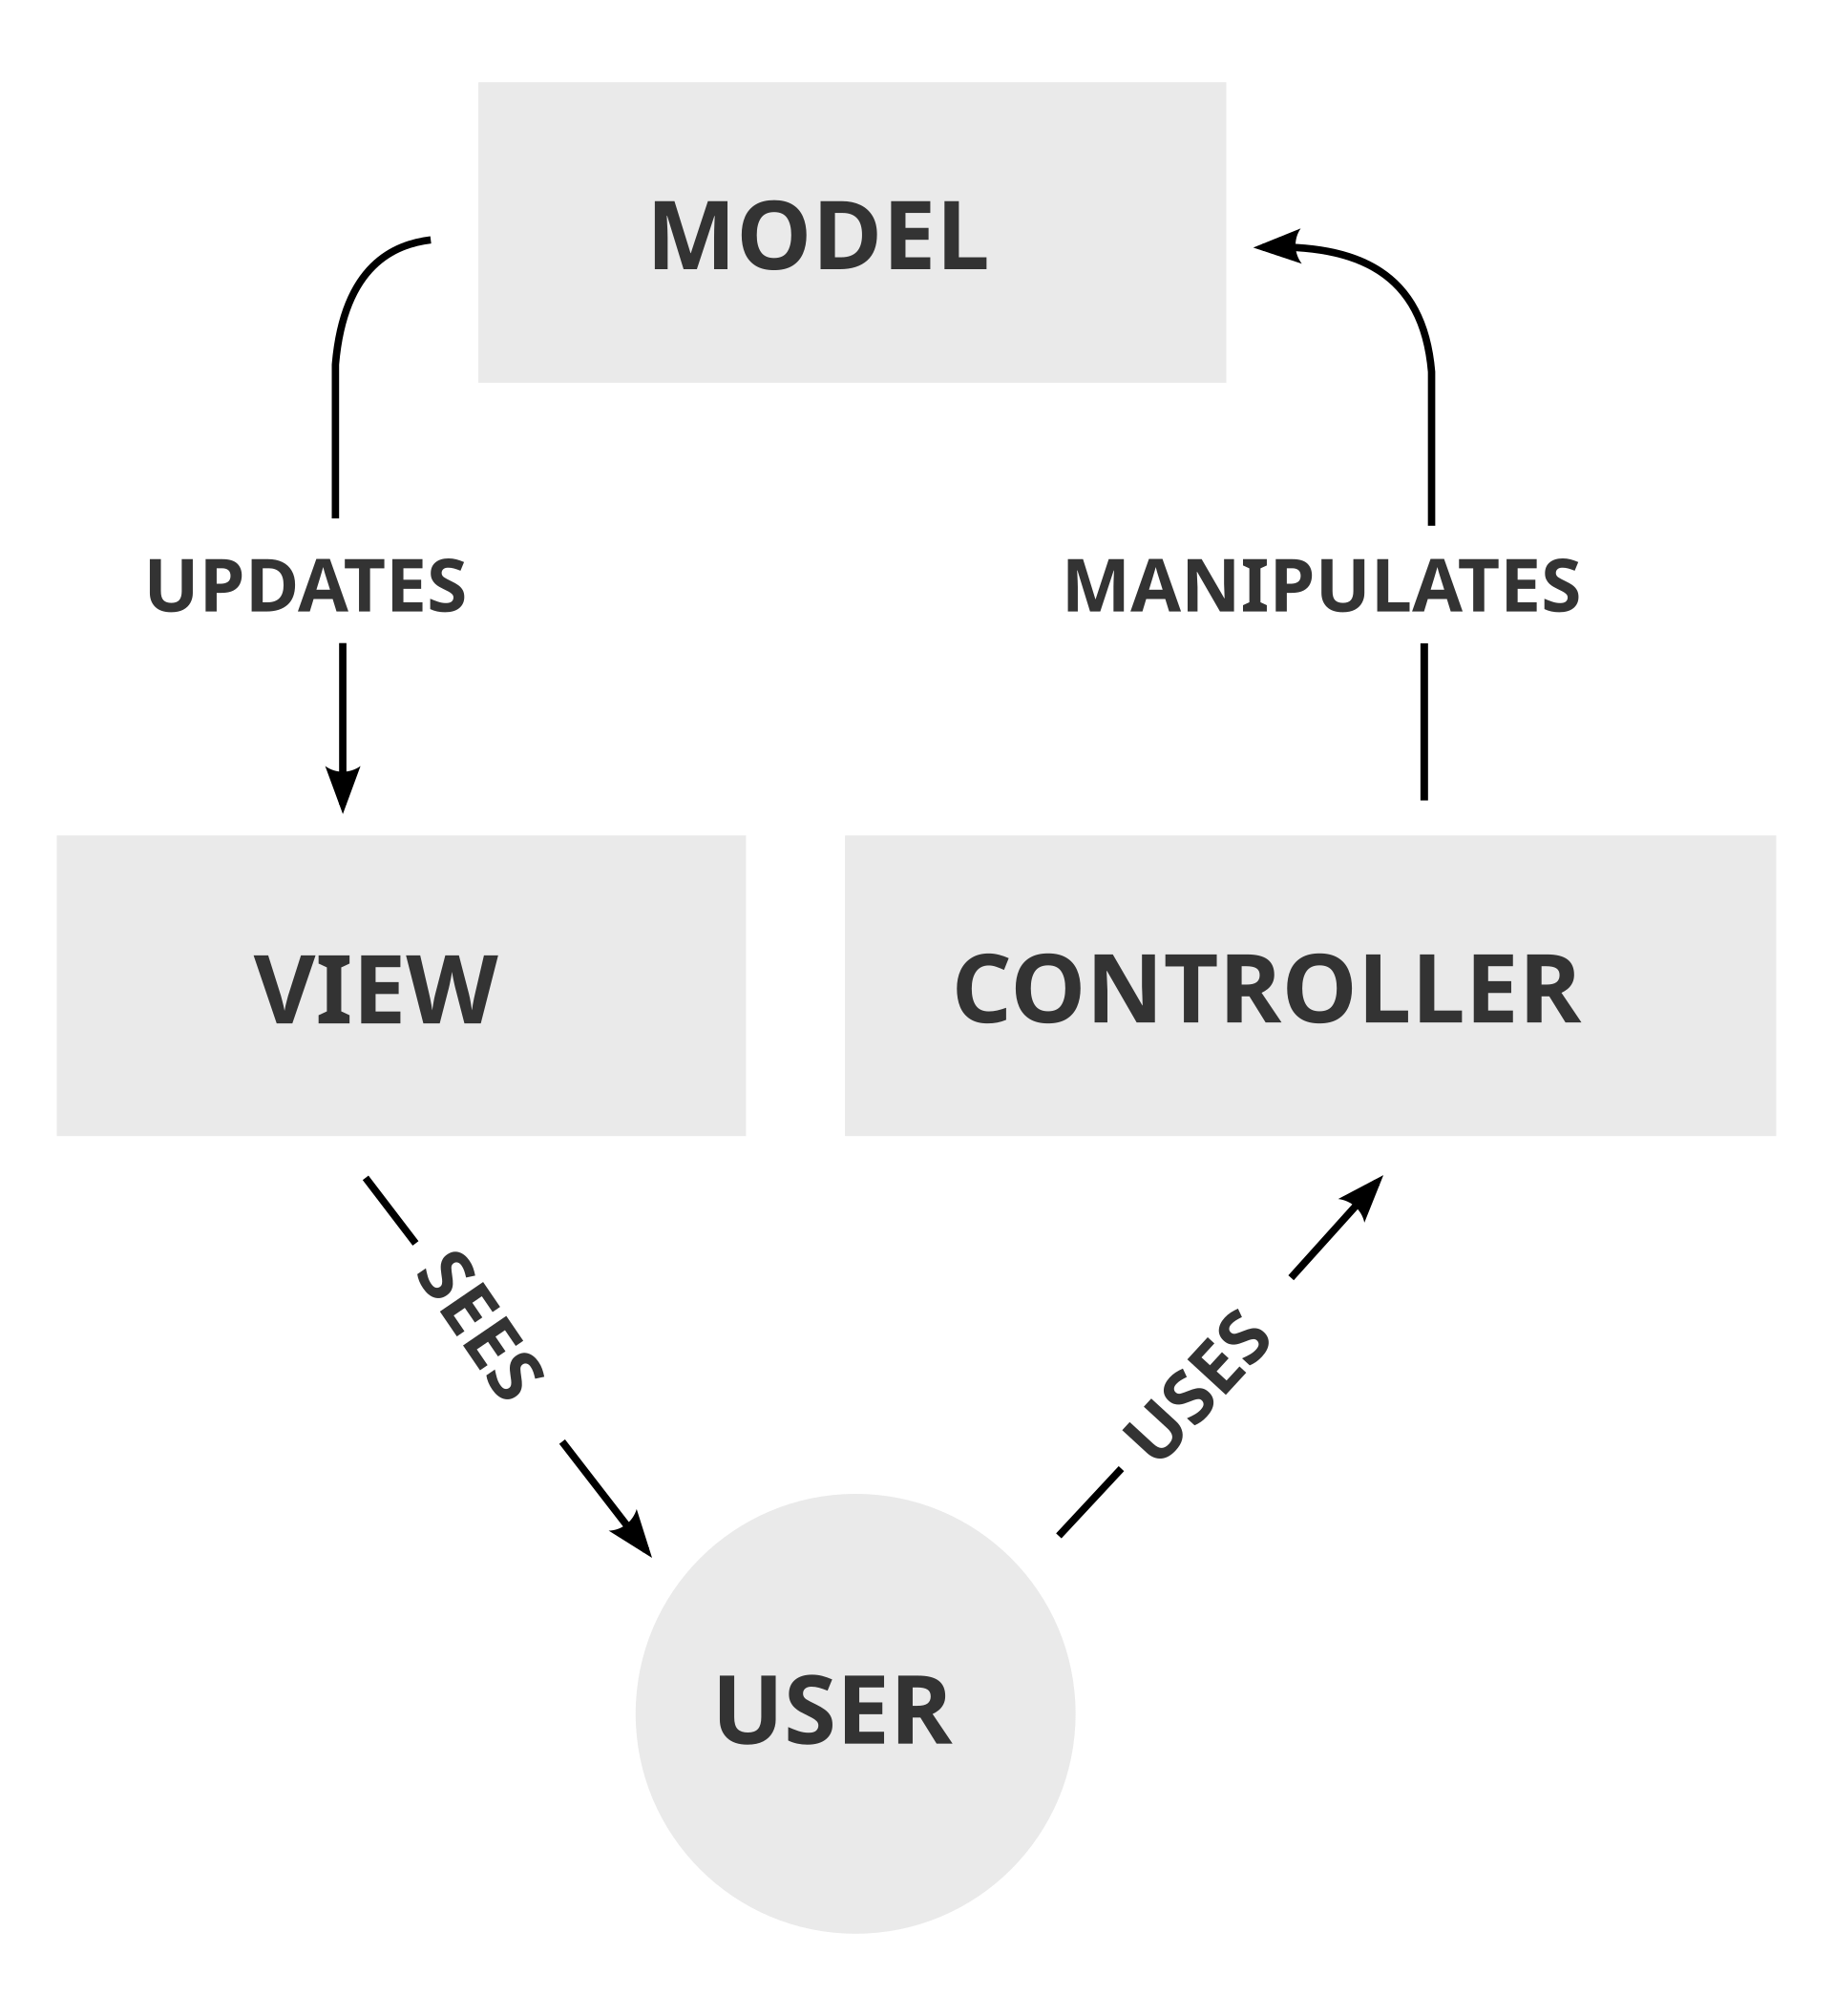
\includegraphics[width=0.7\textwidth]{graphics/MVC-Process.svg.png}
	\caption{\en{MTC} μοντέλο}
\end{figure}

\FloatBarrier

\subsection{\en{Django MTV} }

Παρόλο που το \en{Django} ακολουθεί το μοτίβο \en{MVC}, προτιμά να χρησιμοποιεί τη δική του λογική στην υλοποίηση. Το \en{framework} αναλαμβάνει το \en{Controller} 
μέρος του \en{MVC} και αφήνει τα περισσότερα από τα "καλά" να γίνονται στο \en{Model-Template-View (MTV)}.
Αυτός είναι ο λόγος που το \en{Django} συχνά αναφέρεται ως \en{MTV framework}.



\subsection{Χρήση του \en{MTV} στην εφαρμογή}

Η εφαρμογή διαχείρισης δικτύου έχει υλοποιηθεί με βάση το 
αρχιτεκτονικό μοτίβο \en{MVC (Model-View-Controller)}, το οποίο 
εξασφαλίζει τη σαφή οργάνωση της λειτουργικότητας της εφαρμογής σε 
τρία επίπεδα: το μοντέλο για τη διαχείριση των δεδομένων, τα πρότυπα 
για την παρουσίαση των πληροφοριών στον χρήστη και τις προβολές για 
τη διασύνδεση των χρηστών με τα δεδομένα και την παρουσίασή τους.
Το μοντέλο αποτελεί τον πυρήνα της εφαρμογής και διαχειρίζεται τα 
δεδομένα που σχετίζονται με τις δικτυακές συσκευές. 

Το βασικό μοντέλο που χρησιμοποιείται εδώ είναι το \en{Device}, 
το οποίο αναπαριστά συσκευές όπως δρομολογητές και \en{switches}, 
αποθηκεύοντας πληροφορίες όπως η διεύθυνση του \en{host}, το όνομα 
χρήστη και ο κωδικός πρόσβασης, η πλατφόρμα της συσκευής 
και πρόσθετα στοιχεία ασφαλείας. Το \en{Device} είναι συνδεδεμένο με 
τη βάση δεδομένων της εφαρμογής και παρέχει τις βασικές λειτουργίες 
για την εισαγωγή, ανάγνωση, επεξεργασία και διαγραφή δεδομένων. 
Αυτή η δομή επιτρέπει την κεντρική διαχείριση όλων των δεδομένων που 
απαιτούνται για την ομαλή λειτουργία της εφαρμογής.

Για την παρουσίαση των δεδομένων στον χρήστη, χρησιμοποιούνται αρχεία 
\en{HTML} ως πρότυπα. Αυτά τα αρχεία λειτουργούν ως δυναμικές σελίδες 
που δημιουργούνται με τη γλώσσα \en{Django Template}, εξασφαλίζοντας 
την απεικόνιση των δεδομένων με τρόπο φιλικό προς τον χρήστη. 
Για παράδειγμα, τα πρότυπα χρησιμοποιούνται για την εμφάνιση της λίστας των συσκευών, παρέχοντας λεπτομέρειες για κάθε μία από αυτές, καθώς και για την προβολή στατιστικών ή ρυθμίσεων. Επιπλέον, τα πρότυπα προσαρμόζονται ανάλογα με τα δεδομένα που αντλούνται από το μοντέλο, ώστε να παρέχουν ενημερωμένες πληροφορίες, όπως αποτελέσματα εκτέλεσης εντολών ή την κατάσταση μιας συσκευής.

Οι προβολές της εφαρμογής(\en{views.py}) είναι συναρτήσεις \en{Python} που συνδέουν 
τα αιτήματα των χρηστών με τα δεδομένα και την παρουσίαση. 
Όταν ένας χρήστης κάνει μια ενέργεια, όπως το να ζητήσει την προβολή 
μιας λίστας συσκευών, η αντίστοιχη προβολή λαμβάνει το αίτημα, 
επικοινωνεί με το μοντέλο για να ανακτήσει τα δεδομένα και στη 
συνέχεια τα περνάει στο κατάλληλο πρότυπο. Όλες οι λειτουργικές δυνατότητες της εφαρμογής μας υλοποιούνται μέσα στη σελίδα \en{views.py}.
Το πρότυπο δημιουργεί τη σελίδα \en{HTML} που θα επιστραφεί στον χρήστη, περιέχοντας όλες τις πληροφορίες που ζήτησε. Για παράδειγμα, αν ένας χρήστης θέλει να δει τα στατιστικά μιας συγκεκριμένης συσκευής, η προβολή θα αντλήσει τα απαραίτητα δεδομένα από το μοντέλο και θα τα επιστρέψει στον χρήστη μέσα από ένα προσαρμοσμένο πρότυπο.

Με τον τρόπο αυτό, το μοτίβο \en{MVC} εξασφαλίζει την αποτελεσματική 
λειτουργία της εφαρμογής, διαχωρίζοντας τις ευθύνες ανάμεσα στη 
διαχείριση των δεδομένων, την παρουσίαση τους και την επικοινωνία με τον χρήστη. Η οργάνωση αυτή καθιστά την εφαρμογή ευέλικτη και εύκολη στη συντήρηση, ενώ παράλληλα βελτιώνει την εμπειρία χρήσης, παρέχοντας ένα λειτουργικό και φιλικό περιβάλλον διαχείρισης δικτυακών συσκευών
Στο σχήμα 5.2 παρουσιάζεται διάγραμμα απεικόνισης της βασικής αρχιτεκτονικής της εφαρμογής.

\begin{figure}[h]
	\centering
	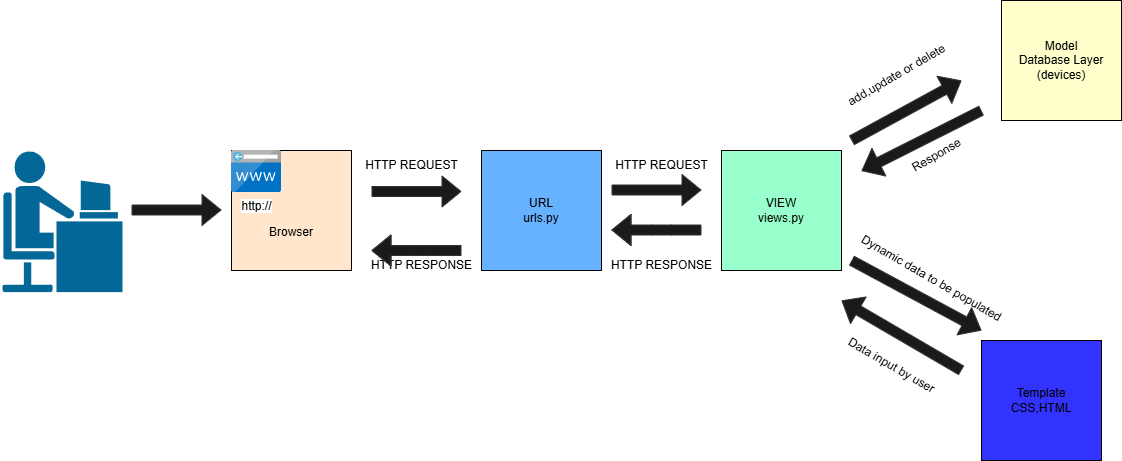
\includegraphics[width=0.7\textwidth]{graphics/MTV.drawio.png}
	\caption{Διαγραμματική απεικόνιση της εφαρμογής}
\end{figure}



\section{Εικονικό Περιβάλλον Δικτύου \en{GNS3 –Testbed}}


Το τοπικό περιβάλλον ανάπτυξης πάνω στο οποίο δοκιµάστηκε η εφαρµογή είναι \en{Linux}, \en{Ubuntu} 22.04.2 \en{LTS} η οποία εικονοποιήθηκε πάνω σε λειτουργκό \en{Windows} ως \en{WSL2}[11]. Το \en{Windows Subsystem for Linux version 2}[11] είναι µια τεχνολογία της \en{Microsoft} που επιτρέπει στους χρήστες \en{Windows} να τρέχουν \en{Linux} περιβάλλοντα απευθείας στο λειτουργικό σύστηµα \en{Windows}, χωρίς την ανάγκη για εξοµοιωτές ή εικονικές µηχανές. Είναι η δεύτερη έκδοση του \en{Windows Subsystem for Linux} και αποτελεί σηµαντική βελτίωση σε σχέση µε την πρώτη έκδοση \en{WSL1}. Το \en{WSL 2} χρησιµοποιεί την τεχνολογία εικονικοποίησης (\en{virtualization}) για να τρέχει έναν πραγµατικό πυρήνα \en{Linux} µέσα σε µια ελαφριά εικονική µηχανή βοηθητικών λειτουργιών (\en{utility VM}). Αυτό επιτρέπει στο \en{WSL 2} να προσφέρει καλύτερη απόδοση, πλήρη συµβατότητα µε τις λειτουργίες \en{Linux} και πρόσβαση σε εργαλεία όπως το \en{Docker}.


Το \en{WSL2} αξιοποιήθηκε διότι παρέχει τη δυνατότητα λειτουργίας ενός 
περιβάλλοντος \en{Linux} μέσα σε έναν υπολογιστή με λειτουργικό 
σύστημα \en{Windows}, χωρίς να απαιτείται η χρήση ενός \en{Type B Hypervisor}. 
Αυτό καθιστά τη διαδικασία πιο ελαφριά και αποδοτική, επιτρέποντας τη 
δημιουργία και εκτέλεση του \en{Django server} και τη διαχείριση των 
απαιτήσεων που περιλαμβάνονται στο αρχείο \en{requirements.txt} με έναν πιο οργανωμένο και σταθερό τρόπο.

Το αρχείο \en{requirements.txt}[16] είναι ένα αρχείο το οποίο περιέχει τις βιβλιοθήκες της \en{Python} που θα χρησιμοποιήσουμε στην εφαρμογή μας. Είναι ένα \en{text} αρχείο το οποίο περιέχει όλα εκείνα τα στοιχεία του λογισμικού τα οποία είναι απαραίτητα προκειμένου να τρέξει η εφαρμογή μας. Με τη βοήθεια του \en{package manager} της \en{Python} το \en{pip} μπορούμε εύκολα να εγκαταστήσουμε με μία εντολή όλες τις βιβλιοθήκες που έχουμε βάλει μέσα σε αυτό το \en{text} αρχείο. Με την εντολή αυτή \en{pip install -r requirements.txt} εγκαθιστούμε αυτόματα όλο το απαραίτητο λογισμικό προκειμένου να τρέξει η εφαρμογή μας.

Η εξοικείωσή μου με περιβάλλοντα \en{Unix} έπαιξε καθοριστικό ρόλο 
στο να επιλέξω να φτιάξω το περιβάλλον αυτό, καθώς το \en{WSL2} προσφέρει μια 
εμπειρία χρήσης που μοιάζει πολύ με αυτή ενός πλήρους \en{Linux} 
συστήματος. Αυτή η προσέγγιση επέτρεψε τη χρήση γνωστών εργαλείων και 
πρακτικών ανάπτυξης, ενώ ταυτόχρονα αξιοποίησε τη συμβατότητα του \en{Windows} 
οικοσυστήματος το οποίο χρειάστηκε για την εγκατάσταση του \en{GNS3}. Έτσι, επιτεύχθηκε η δημιουργία ενός τοπικού περιβάλλοντος 
ανάπτυξης που συνδυάζει την ευελιξία και τη σταθερότητα των \en{Unix} 
συστημάτων με την ευκολία πρόσβασης που παρέχει το λειτουργικό σύστημα \en{Windows}.

Το γεγονός ότι το \en{WSL2} αποτελεί ένα \en{Linux} περιβάλλον που εκτελείται πάνω σε λειτουργικό σύστημα \en{Windows} είχε καθοριστική σημασία για την παρούσα υλοποίηση. Αυτό οφείλεται στο ότι τόσο το \en{GNS3} όσο και το \en{VirtualBox} εγκαταστάθηκαν στο \en{Windows} περιβάλλον, ενώ το \en{WSL2} αξιοποιήθηκε αποκλειστικά για την ανάπτυξη της εφαρμογής \en{Django}. Αυτή η διάκριση στη χρήση των εργαλείων επέτρεψε την ομαλή ενσωμάτωση του \en{Linux} περιβάλλοντος στο συνολικό σύστημα, διατηρώντας παράλληλα τη συμβατότητα με τις απαιτήσεις της προσομοίωσης δικτύου.

\subsection{Σχεδίαση Τοπολογίας Δικτύου}

Η ανάπτυξη του \en{Testbed} βασίστηκε στη λογική ότι οι συσκευές που εκτελούνται στο \en{GNS3 VM} θα πρέπει να μπορούν να αλληλεπιδρούν με το τοπικό περιβάλλον \en{WSL2}[19]. Για να επιτευχθεί αυτός ο στόχος, ακολουθήθηκε μια συγκεκριμένη μεθοδολογία, η οποία περιλαμβάνει διαδοχικά βήματα.
Το πρώτο και θεμελιώδες βήμα ήταν η εγκατάσταση των απαραίτητων λογισμικών εργαλείων, τα οποία έχουν ήδη παρουσιαστεί στο θεωρητικό υπόβαθρο. Η διαδικασία δημιουργίας του \en{testbed} αποδείχθηκε ιδιαίτερα απαιτητική, γι' αυτό και θα εξηγήσουμε ορισμένες βασικές αρχές που διέπουν τη λειτουργία του, ώστε να γίνει πιο κατανοητή.
Όπως αναφέρθηκε στο προηγούμενο κεφάλαιο, έχουμε ήδη εγκαταστήσει το \en{GNS3}, το \en{GNS3 VM} στο \en{VirtualBox}, και πλέον είμαστε έτοιμοι να διαμορφώσουμε το περιβάλλον όπου οι συσκευές της \en{Cisco}, που εκτελούνται στο \en{GNS3 VM}, θα μπορούν να επικοινωνούν με το \en{WSL2}, το οποίο αποτελεί και το βασικό λειτουργικό σύστημα του πειραματικού μας περιβάλλοντος.


Λόγω των περιορισμένων υπολογιστικών πόρων που διατίθενται στο πλαίσιο αυτής της διπλωματικής εργασίας, η τοπολογία που χρησιμοποιήθηκε είναι απλή, όπως φαίνεται και στο Σχήμα 5.3. Συγκεκριμένα, η δομή του \en{testbed} περιλαμβάνει πρώτον έναν κόμβο \en{Cloud}, ο οποίος επιτρέπει τη δικτυακή αλληλεπίδραση μεταξύ των συσκευών του \en{GNS3 VM} και του \en{WSL2} και μία συσκευή δοκιμών, που χρησιμοποιείται για την αξιολόγηση της συνδεσιμότητας και της επικοινωνίας στο προτεινόμενο περιβάλλον. Επιλέχθηκε αυτή η τοπολογία διότι αυτή είναι ικανή να μας προσφέρει με το ελάχιστο δυνατό υπολογιστικό κόστος το απαραίτητο περιβάλλον που θα τεστάρουμε.
Με αυτήν την προσέγγιση, διασφαλίζεται η σωστή λειτουργία του \en{testbed}, καθιστώντας εφικτή τη μελέτη και την ανάλυση της επικοινωνίας μεταξύ των εικονικών και των φυσικών συσκευών.

\FloatBarrier

\begin{figure}[htb]
	\centering
	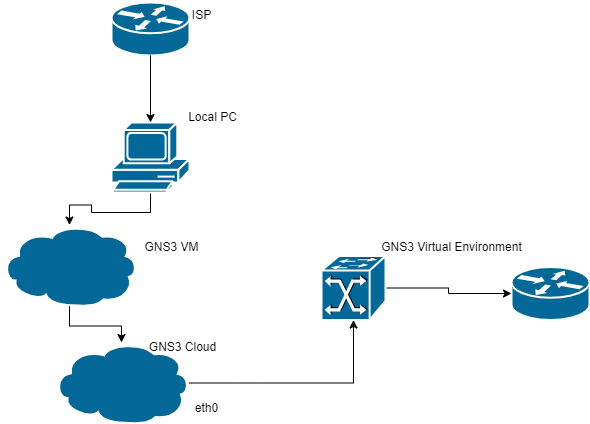
\includegraphics[width=0.7\textwidth]{graphics/diagram.drawio.png}
	\caption{\en{Local PC-GNS3VM-CISCO IOS Connection Architecture} }
\end{figure}

\FloatBarrier

Το \en{GNS3 cloud node} μας δίνει τη δυνατότητα να συνδέσουμε τις συσκευές μας που τρέχουν στο \en{GNS3 VM} με το τοπικό μας δίκτυο. Για να γίνει αυτό ρυθμίζουμε το \en{cloud node} έτσι ώστε to \en{eth0 interface} του να δώσει \en{ip} διεύθυνση μέσα από το \en{DHCP} πρωτόκολλο στα \en{devices} μας. Με αυτόν τον τρόπο έχουμε απευθείας πρόσβαση σε αυτά μέσα από το τοπικό μας δίκτυο.

Για την παραμετροποίηση του \en{Cloud Node}, ρυθμίζουμε το \en{interface} που συνδέεται με τη συσκευή, ακολουθώντας την παρακάτω διαδικασία. Αρχικά, συνδέουμε το \en{interface eth0} του \en{Cloud Node} με το αντίστοιχο \en{eth0} της συσκευής, όπως φαίνεται στην 5.4 εικόνα. 

\FloatBarrier

\begin{figure}[htb]
	\centering
	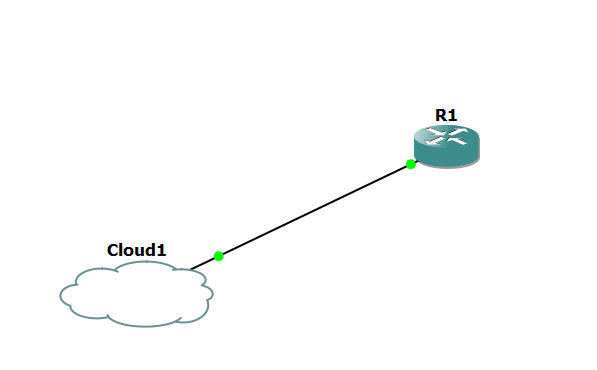
\includegraphics[width=0.7\textwidth]{graphics/CISCO_CLOUD.png}
	\caption{\en{CLOUD NODE With CISCO Node Connection} }
\end{figure}

\FloatBarrier

\noindent Η σύνδεση πραγματοποιείται μέσω της επιλογής του \en{interface} από το \en{Configuration Menu} του \en{Cloud Node}. Συγκεκριμένα, κάνουμε δεξί κλικ στο \en{Cloud Node}, επιλέγουμε "Παραμετροποίηση" και στη συνέχεια προσθέτουμε το \en{eth0} ως τη διεπαφή επικοινωνίας του τοπικού δικτύου με τον διακομιστή όπως φαίνεται στην εικόνα 5.5.

\FloatBarrier

\begin{figure}[htb]
	\centering
	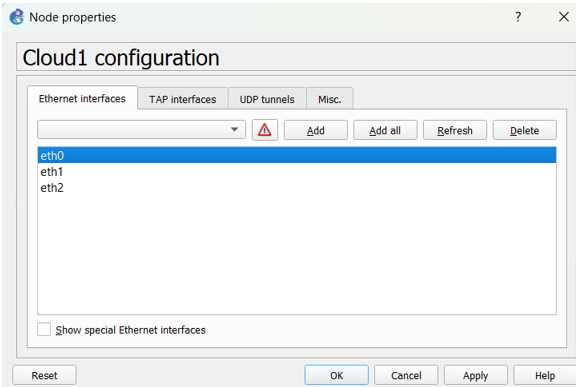
\includegraphics[width=0.7\textwidth]{graphics/CLOUD_NODE_CONFIGURATION.png}
	\caption{\en{CLOUD NODE Configuration} }
\end{figure}

\FloatBarrier


\noindent Η επιλογή του \en{eth0} είναι καθοριστικής σημασίας, καθώς στο \en{GNS3 VM} το συγκεκριμένο \en{interface} είναι ήδη προρυθμισμένο για αυτήν τη λειτουργία, διασφαλίζοντας έτσι την ορθή επικοινωνία του τοπικού δικτύου με τον διακομιστή. Γιατί όμως επιλέγουμε το \en{eth0} στο σχήμα 5.4 και όχι το \en{eth1} ή το \en{eth2}.

Επιλέγουμε το \en{eth0} στο \en{Cloud node} διότι αυτό ανήκει στο δίκτυο της Γεφυρωμένης Κάρτας Δικτύου που επιλέξαμε για το \en{GNS3 VM}. Στην εικόνα παρακάτω(Σχήμα 5.6) βλέπουμε την κάρτα δικτύου του \en{GNS3 VM}.

\FloatBarrier

\begin{figure}[htb]
	\centering
	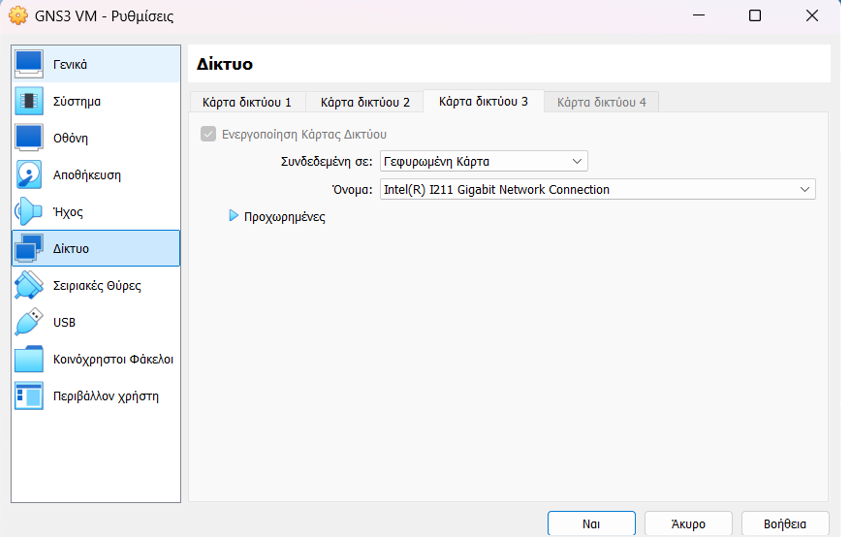
\includegraphics[width=0.7\textwidth]{graphics/GNS3_network_adapter.png}
	\caption{\en{GNS3 VM} κάρτα δικτύου }
\end{figure}

\FloatBarrier

\noindent Προκειμένου να φτιάξουμε την κάρτα δικτύου αυτή μέσα από τα εργαλεία του \en{Vbox} πατάμε Δημιουργία \en{Host-only Networks}
και ρυθμίζουμε την κάρτα δικτύου όπως φαίνεται στο σχήμα 5.7. Στο σχήμα φαίνεται ότι όλες οι συσκευές μας θα πρέπει να παίρνουν \en{IP} διεύθυνση από το δίκτυο 192.168.56.0/24


\FloatBarrier

\begin{figure}[htb]
	\centering
	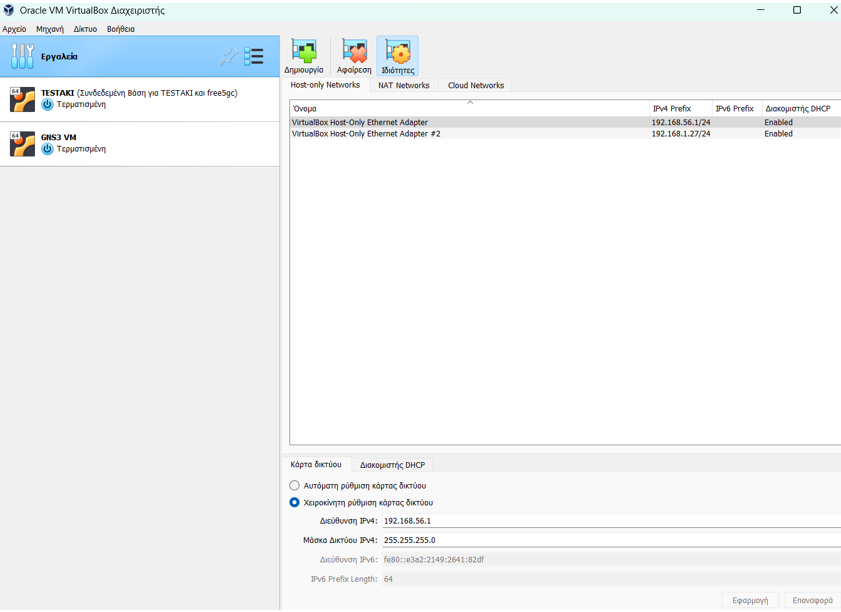
\includegraphics[width=0.7\textwidth]{graphics/GNS3_Network.png}
	\caption{\en{GNS3 VM} δίκτυο }
\end{figure}

\FloatBarrier


\noindent Αφού φτιάξουμε την κάρτα δικτύου του \en{VBox} αυτή μετά φαίνεται αυτόματα στις συνδέσεις δικτύου του υπολογιστή μας όπως στην εικόνα 5.8.

\FloatBarrier

\begin{figure}[htb]
	\centering
	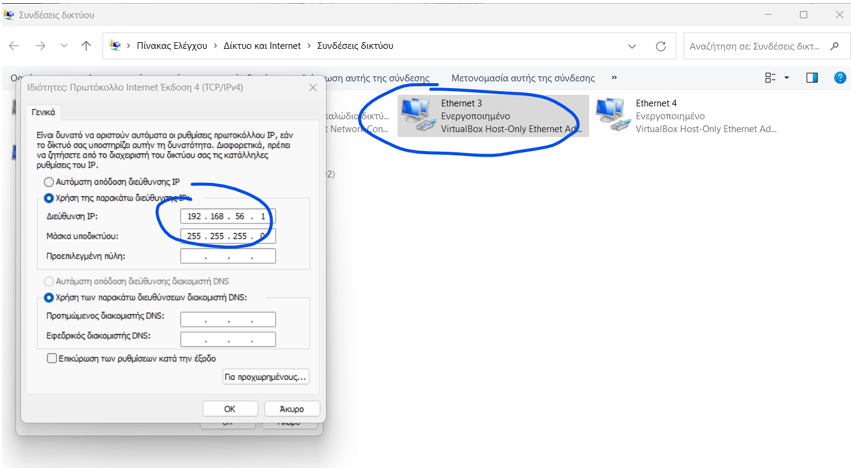
\includegraphics[width=0.7\textwidth]{graphics/windows_host_networking.png}
	\caption{Κάρτα δικτύου στο \en{Windows} λειτουργικό}
\end{figure}

\FloatBarrier

Προκειµένου τώρα οι συσκευές αυτές να µπορέσουν να µιλήσουν µε το τοπικό µας δίκτυο θα πρέπει να τους ορίσουµε \en{IP} διευθύνσεις . Συνεπώς με αυτήν την παραμετροποίηση όταν παραμετροποιήσουμε και τη δικτυακή συσκευή να παίρνει \en{IP} διεύθυνση από αυτό το τοπικό δίκτυο τότε θα μπορούμε από το τοπικό δίκτυο να μιλάμε με στις συσκευές μας για τους \en{testing} λόγους.
Προκειμένου να παίρνουν οι συσκευές \en{IP} διεύθυνση από το τοπικό δίκτυο δηλαδή από το εικονικό \en{interface} του \en{Vbox} που δημιουργήσαμε παραπάνω(192.168.56.0/24) κάναμε την παρακάτω παραμετροποίηση.
Στο σχήμα 5.9 φαίνεται η παραμετροποίηση στην δικτυακή συσκευή.

\FloatBarrier

\begin{figure}[htb]
	\centering
	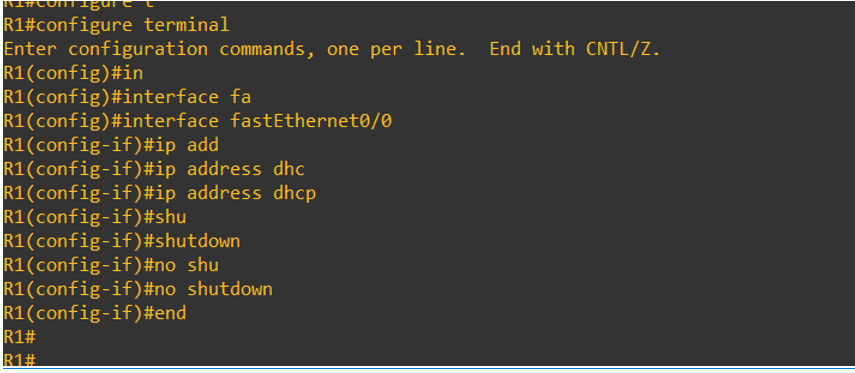
\includegraphics[width=0.7\textwidth]{graphics/cisco_ssh_config_2.png}
	\caption{Παραμετροποίηση στη δικτυακή συσκευή}
\end{figure}

\FloatBarrier

\noindent Στο σχήμα 5.10 φαίνεται η συσκευή να παίρνει σωστά \en{IP} διευθύνση από το 192.168.56.0/24.

\FloatBarrier

\begin{figure}[htb]
	\centering
	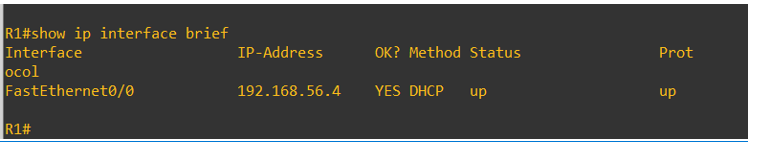
\includegraphics[width=0.7\textwidth]{graphics/cisco_ip_address.png}
	\caption{Κατανομή \en{IP} διευθύνσης}
\end{figure}

\FloatBarrier


\noindent Αφού το \en{interface} πήρε \en{IP} διεύθυνση ελέγχουμε στο τέλος ότι μπορούμε να επικοινωνήσουμε με τη συσκευή όπως στο σχήμα 5.11. Στα σχήματα οι \en{IP} διευθύνσεις μπορεί να είναι διαφορετικές καθώς δοκιμάστηκαν σε διαφορετική φάση. Η ουσία όμως είναι ότι όλες θα παίρνουν \en{IP} διεύθυνση από το δίκτυο 192.168.56.1/24 το οποίο θα αποτελεί και το τελικό δίκτυο πάνω στο οποίο θα αλληλεπιδρούν ο \en{Django Server} με το \en{GNS3 testbed}. Το δίκτυο αυτό είναι κοινό για όλα τα \en{nodes} που βλέπουμε στο Σχήμα 5.3 το οποίο σχεδιάστηκε προκειμένου να γίνει κατανοητή η σχεδίαση.

\FloatBarrier

\begin{figure}[htb]
	\centering
	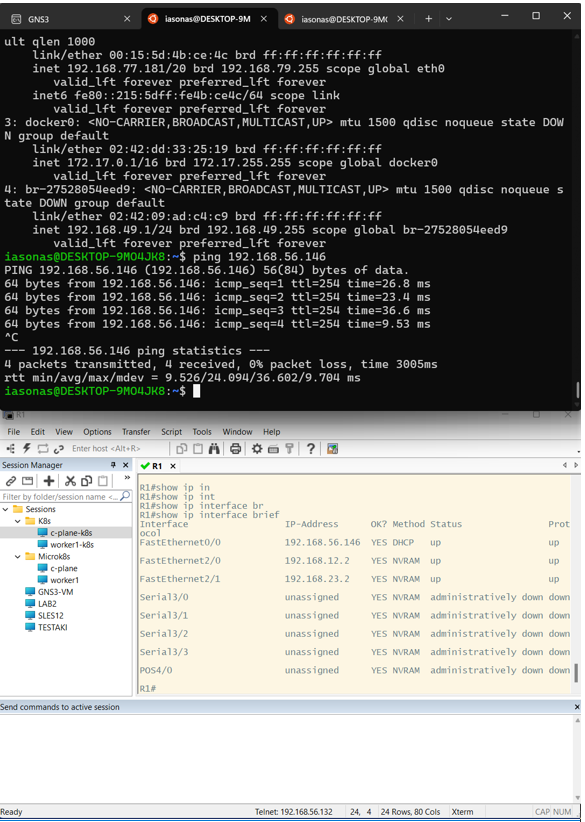
\includegraphics[width=0.7\textwidth]{graphics/ip_connectivity_test.png}
	\caption{\en{IP connectivity test}}
\end{figure}

\FloatBarrier





\subsection{Προσομοίωση Συσκευών \en{Cisco}}

  Προκειμένου να προσομειώσουμε συσκευές της \en{Cisco} το πρώτο βήμα είναι να κατεβάσουμε συγκεκριμένο \en{appliance} απο το \en{GNS3 marketplace}. Αφού το κατεβάσουμε το εισάγουμε στο \en{GNS3} με τον εξής τρόπο: (εικόνα 5.12)

\FloatBarrier

\begin{figure}[htb]
	\centering
	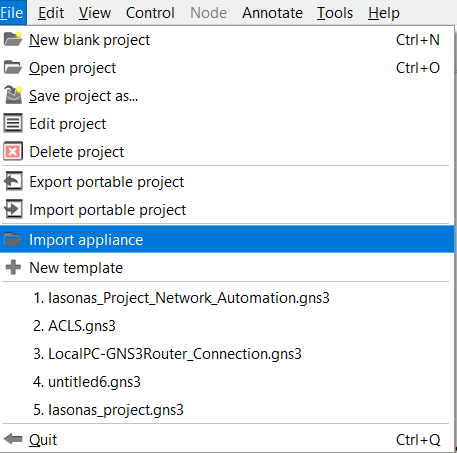
\includegraphics[width=0.7\textwidth]{graphics/import_appliance.png}
	\caption{\en{Import appliance} }
\end{figure}

\FloatBarrier

\noindent Ακολούθως πατάμε \en{Install appliance on the GNS3 VM} και ματσάροντας το \en{filename} του \en{appliance} με το \en{image} που έχουμε μας επιτρέπει να εισάγουμε τη συσκευή. Για να δούμε το \en{filename} στο \en{appliance} ανοίγουμε το αρχείο με έναν \en{editor} και αλλάζουμε το \en{filename} αντίστοιχα οπως στην  εικόνα 5.13.

\FloatBarrier

\begin{figure}[htb]
	\centering
	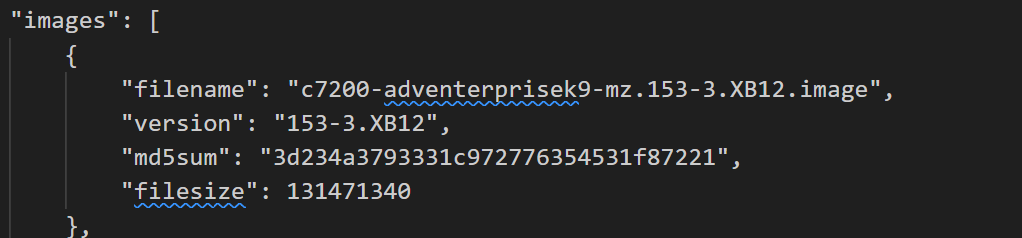
\includegraphics[width=0.7\textwidth]{graphics/appliance_filename.png}
	\caption{\en{filename configuration} }
\end{figure}

\FloatBarrier

Μετά το τέλος της διαδικασίας η συσκευή θα έχει προστεθεί και μπορούμε να την δούμε στην επιλογή \en{Browse all devices}.
Συνεπώς θα μπορούμε να την προσθέσουμε σε τοπολογία και να την κάνουμε να δουλέψει. Για να μπορέσουμε να δουλέψουμε με τη συσκευή θα πρέπει να έχουμε παραμετροποιήσει συγκεκριμένο \en{username},\en{password},\en{secret} καθώς και να τρέχει \en{ssh service}
προκειμένου να μπορούμε να συνδεθούμε μέσα απο το \en{API}. 

Στην  εικόνα 5.14 φαίνεται τι πρέπει να έχει υλοποιηθεί ως προυπόθεση στην εφαρμογή. Φυσικά θεωρούμε δεδομένο ότι έχουν γίνει όλα τα προηγούμενα βήματα καθώς το παρακάτω αφορά μόνο το χρήστη και τον κωδικό του προκειμένου να υλοποιήσει την \en{SSH} σύνδεση.
\FloatBarrier

\begin{figure}[htb]
	\centering
	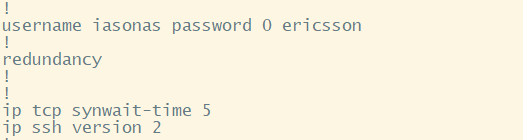
\includegraphics[width=0.7\textwidth]{graphics/ssh.png}
	\caption{\en{ssh and credentials requirements} }
\end{figure}

\FloatBarrier
